\section{Supplemental}
\vfill

\setcounter{figure}{0}
\renewcommand{\thefigure}{S\arabic{figure}}
\setcounter{table}{0}
\renewcommand{\thetable}{S\arabic{table}}

\begin{figure}[!ht]
\centering 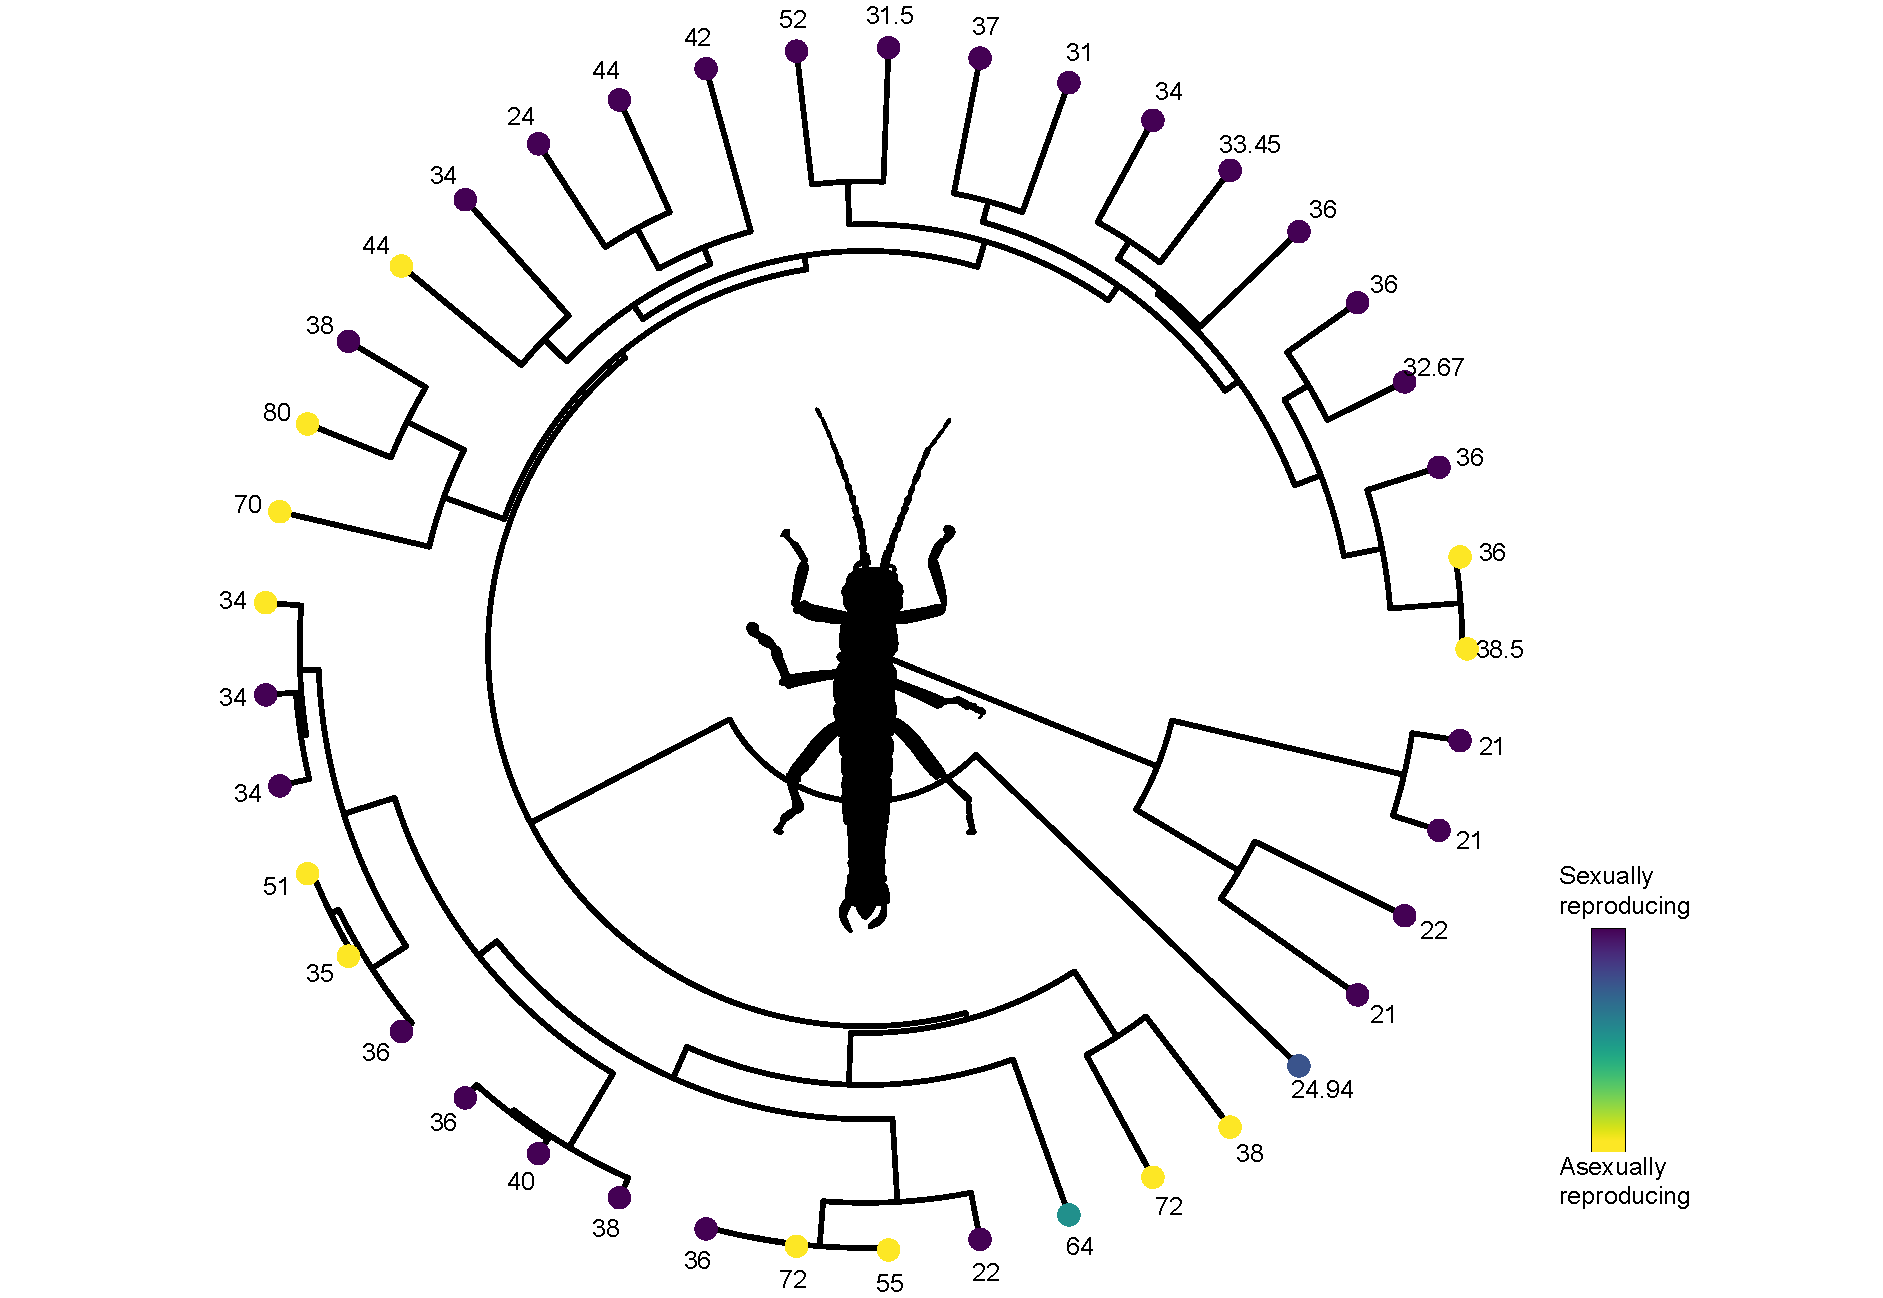
\includegraphics[width=1\textwidth]{figures/phasmatodea_phylogeny.pdf}
\caption{Phylogeny of the insect clade Phasmatodea. Tips are colored according to the mode of reproduction (sexual or asexual). Some lineages show intermediate colours. These are lineages which have both sexual and asexual populations. The shade of colour indicates the probability of observig either reproductive modes in these lineages. The numbers indicate the mean chromosome number for each lineage.}
\label{fig:phas.phylo}
\end{figure}

\begin{figure}
\centering 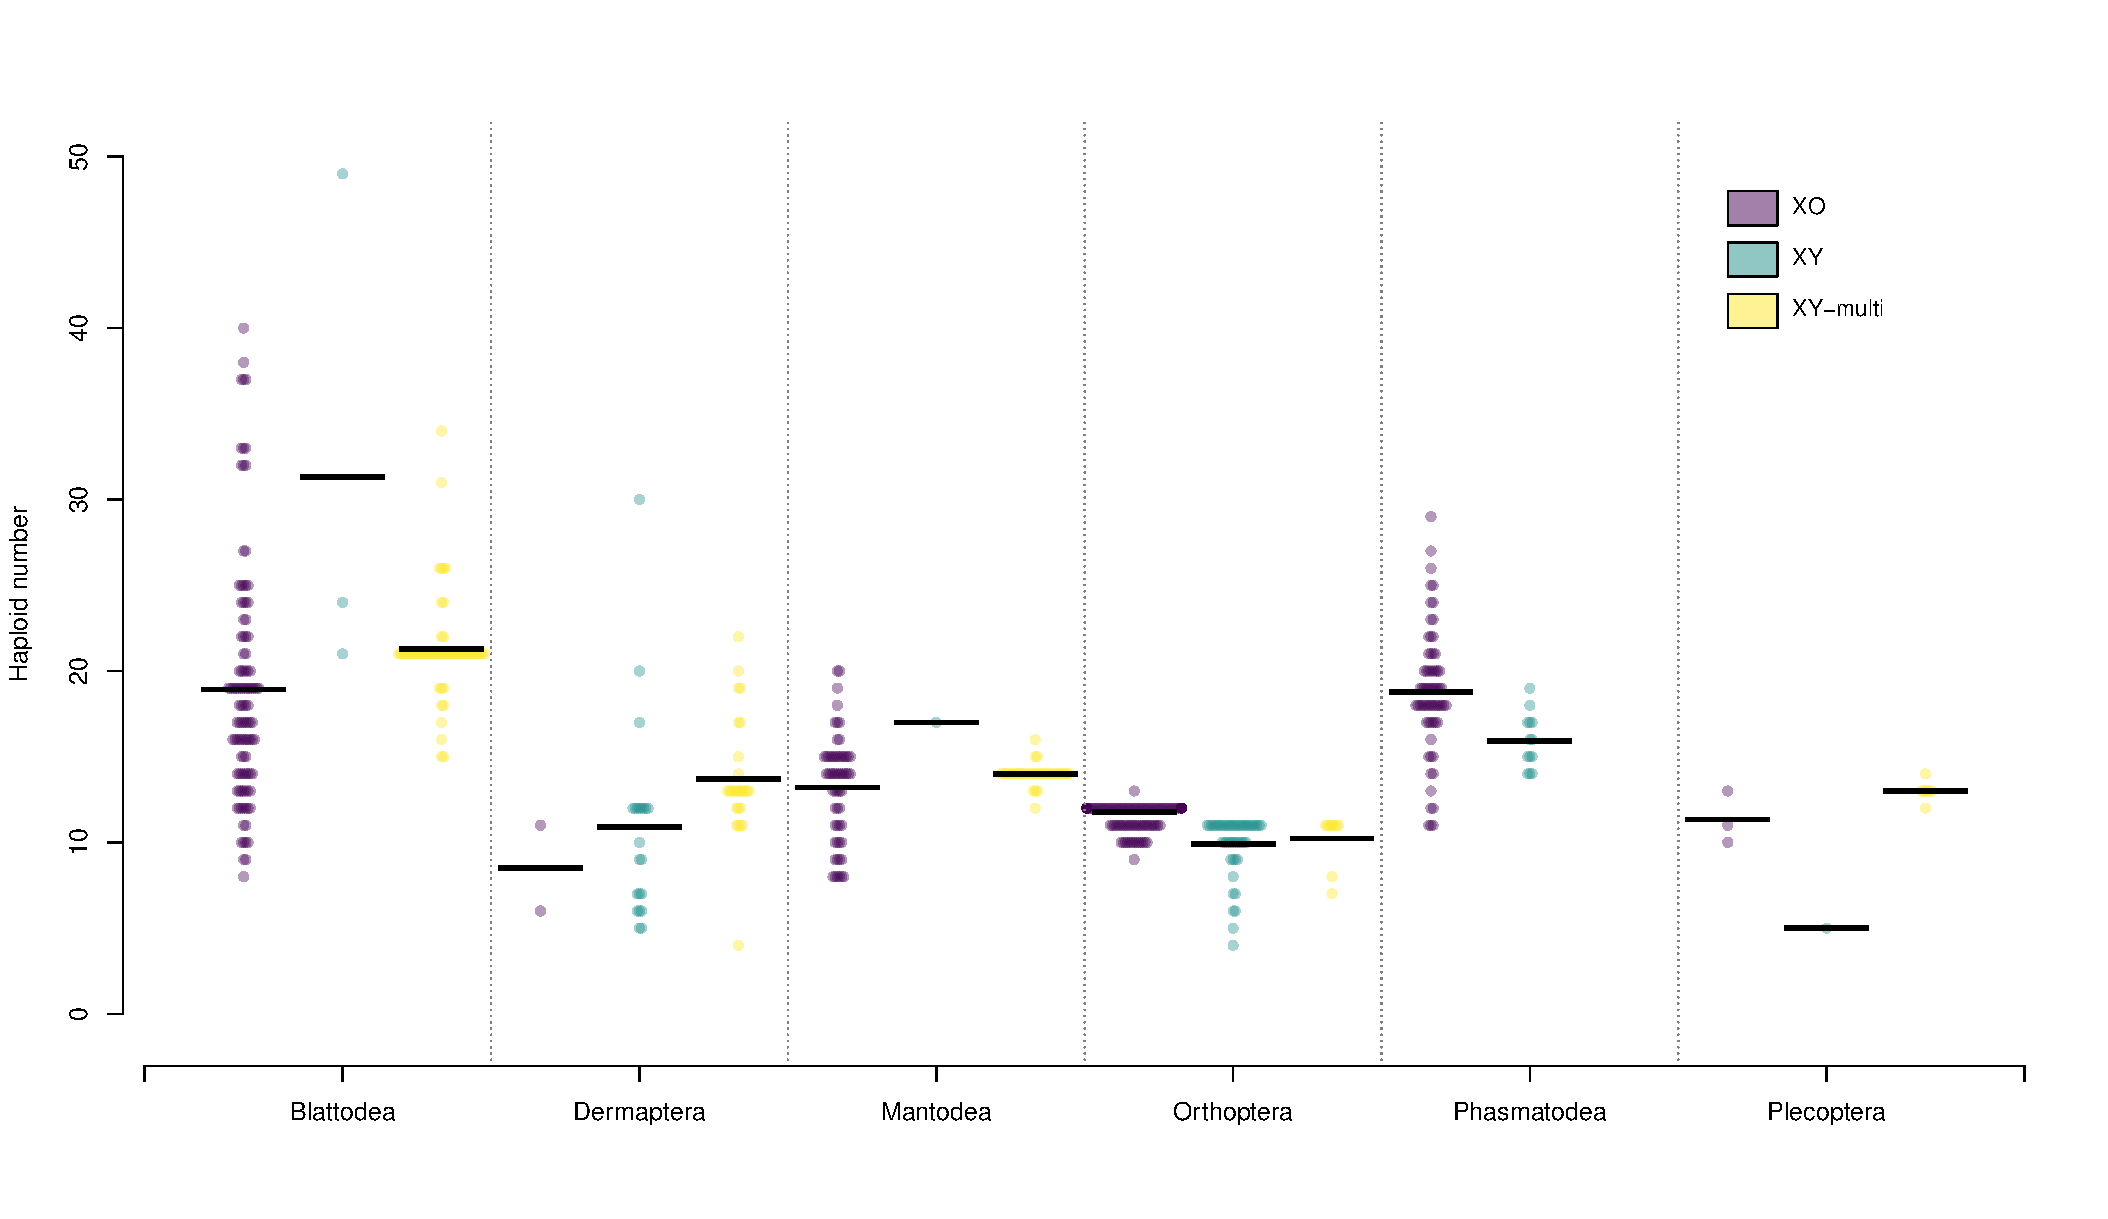
\includegraphics[width=.7\textwidth]{figures/Preliminary_data.pdf}
\caption{
Variation in chromosome numbers with respect to the sex chromosome system in six Polyneoptera orders. Vertical axis indicates the haploid chromosome count. dashed lines represent standard error of the mean.
}
\label{fig:order.plots}
\end{figure}

\begin{figure}
\centering 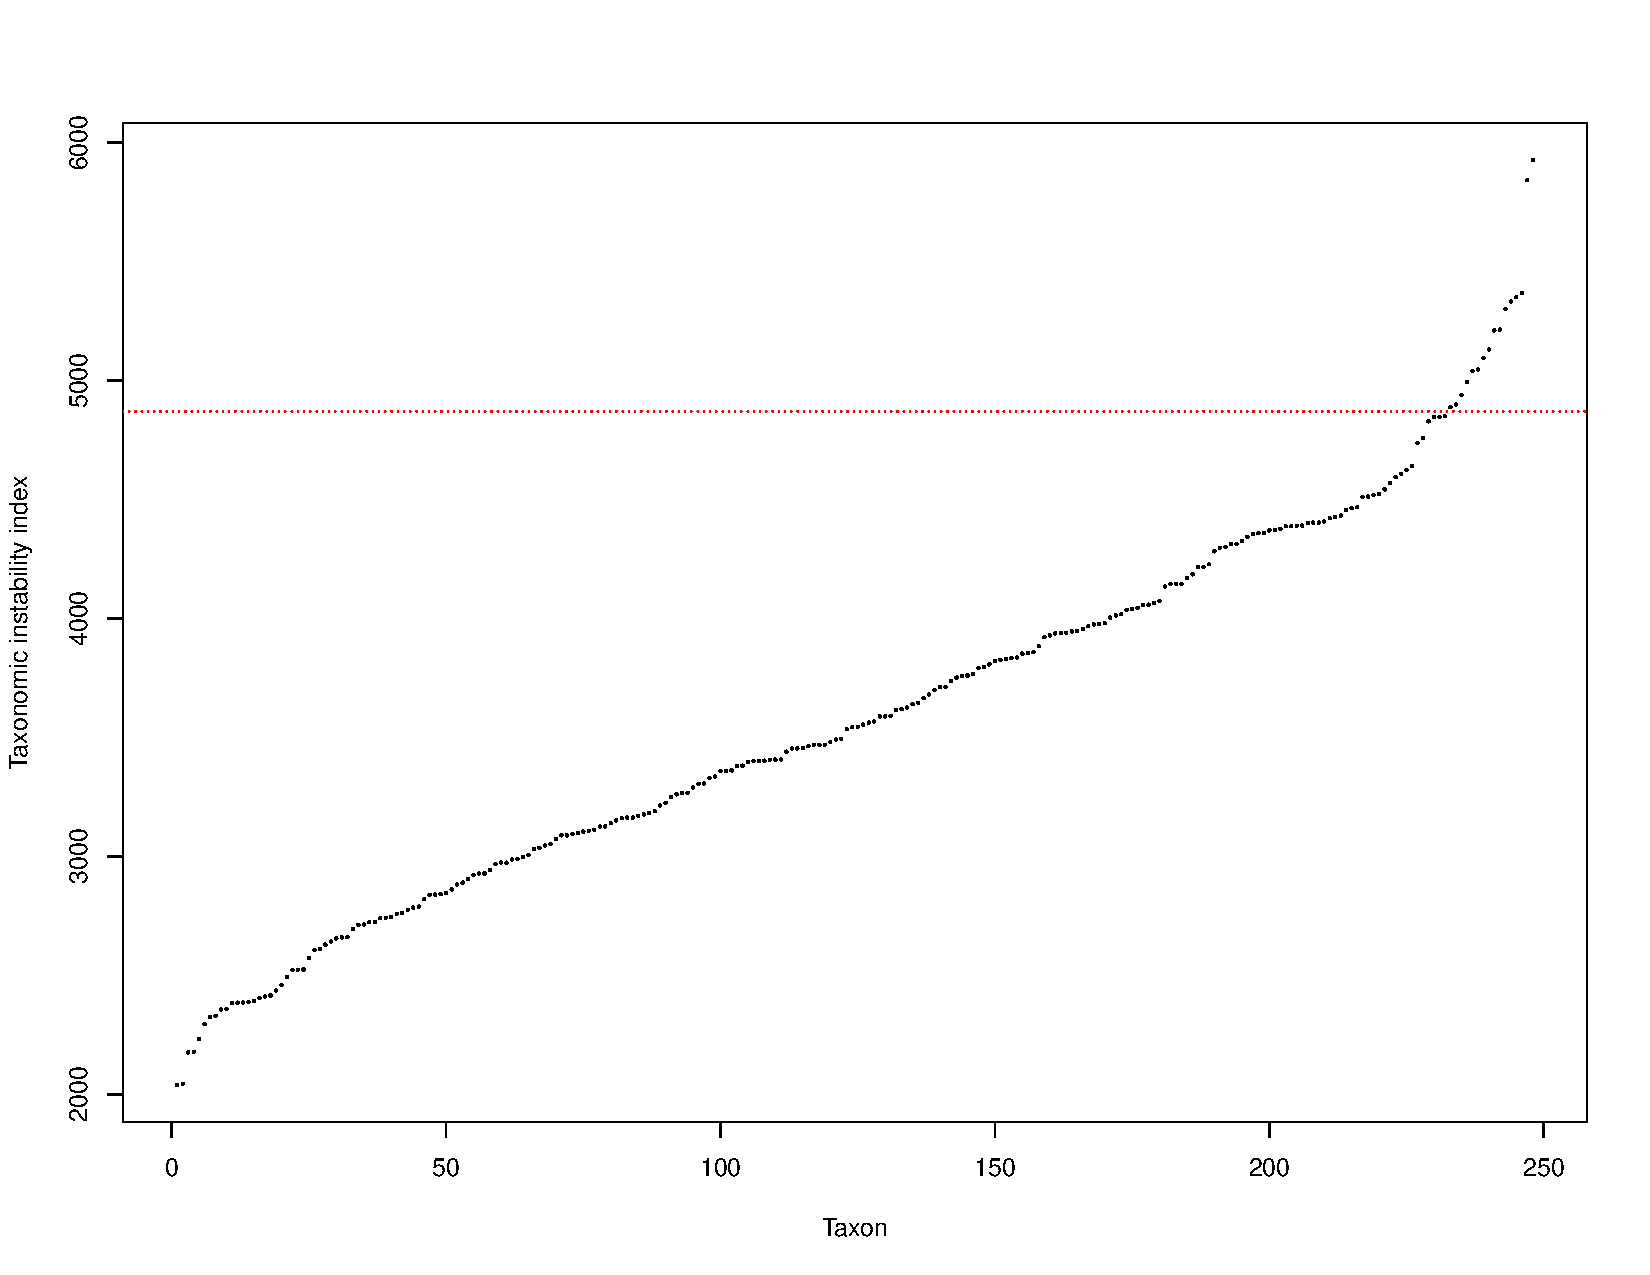
\includegraphics[width=.5\textwidth]{figures/taxonomic_instability_index_plot.pdf}
\caption{
Red dotted line represents the cutoff point of 4780. Roughly about 94\% of the taxa fall below this cutoff point
}
\label{fig:tax.index}
\end{figure}

\begin{figure}
\centering 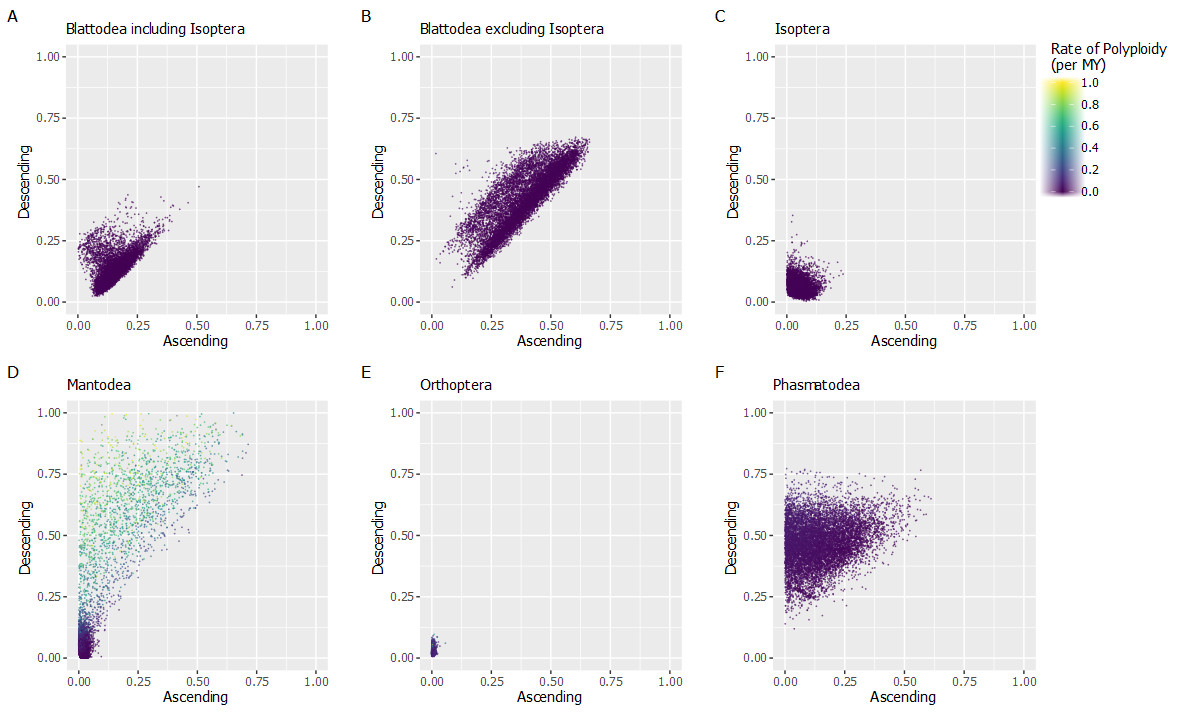
\includegraphics[width=1\textwidth]{figures/rate_estimates.jpg}
\caption{
Rates of chromosome fission (ascending) and fusion (descending) in five orders of Polyneoptera. Here these rates are color coded according to the rate of polyploidy in each order. 
}
\label{fig:rates}
\end{figure}

\begin{figure}
\centering 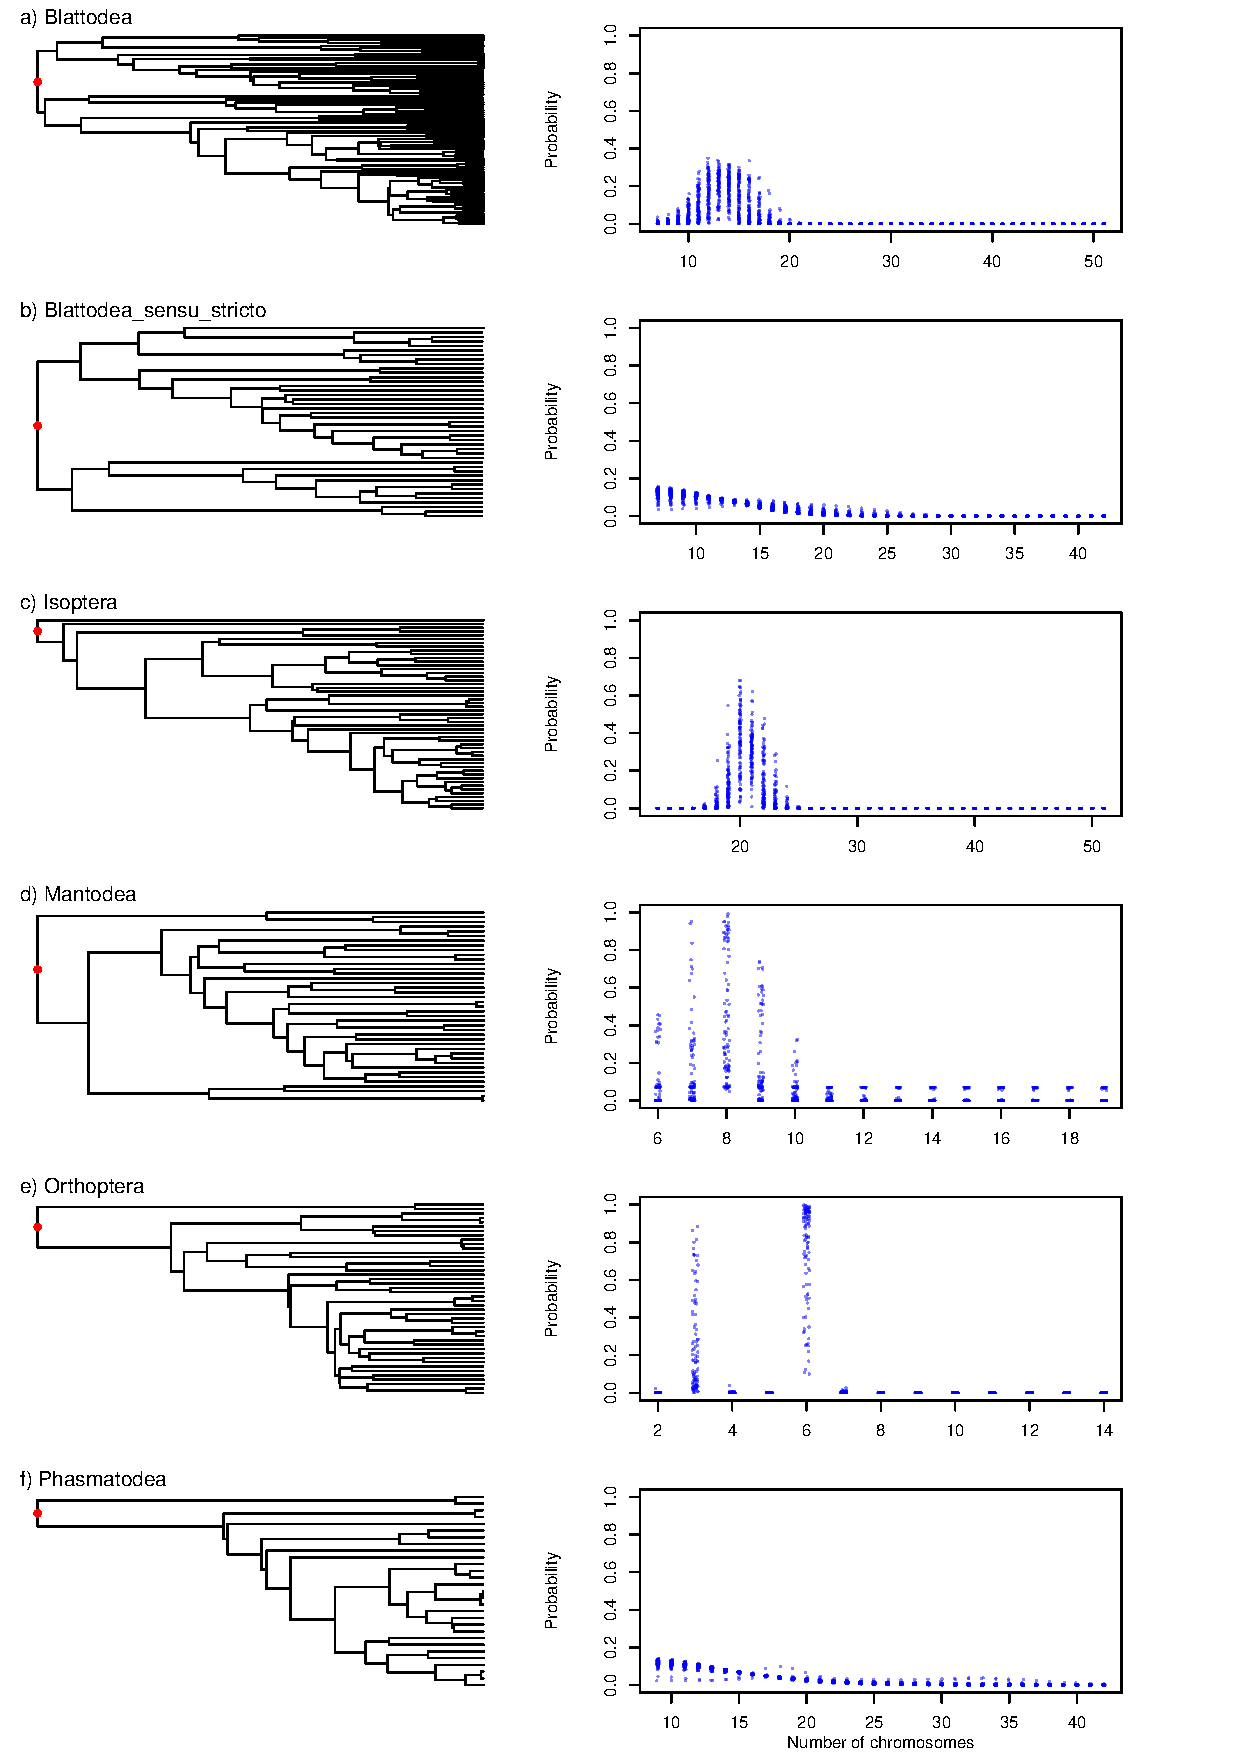
\includegraphics[width=.7\textwidth]{figures/asr_plot.pdf}
\caption{Ancestral states reconstruction of the studied taxa. The root of each clade is indicated by red dot. Except for Orthoptera where we see chromosome numbers three and six as the only inferred ancestral states, we find a normal distribution for ancestral states in all other clades.}
\label{fig:asr}
\end{figure}

\begin{table}[ht]
\begin{tabular}{lcc}
\hline
\textbf{Transition} & \textbf{Mean rate (95\% credible interval)} & \textbf{Mean number of transitions} \\ \hline
XO to XY            & 0.0020 (0.0015 - 0.0026)                    & 15.3                                \\
XY to XO            & 0.0021 (0.0010 - 0.0036)                    & 6.7                                 \\ \hline
\end{tabular}
\caption{Mean transition rates and mean number of transitions obtained from stochastic mapping of sex chromosome transitions}
\label{tab:simmap.summary}
\end{table}

\begin{table}
\centering
\begin{tabular}{ll}
\hline
\textbf{Mean rate (95\% Credible Interval)}  & \textbf{Mean number of transitions} \\ \hline
\multicolumn{1}{c}{0.0063 (0.0052 - 0.0078)} & \multicolumn{1}{c}{9.3}             \\ \hline
\end{tabular}
\caption{Mean rate of transition from sexual reproduction to parthenogenesis and mean number of 
such transitions estimated from stochastic mapping. The transition rate of parthenogenesis to sexual reproducing was set to zero}
\label{tab:phas.simmap.summary}
\end{table}
